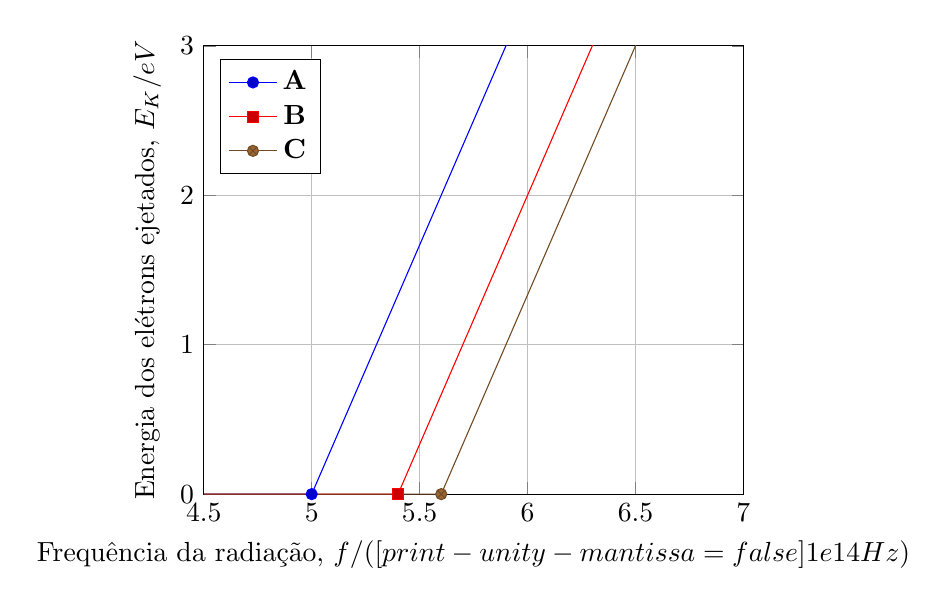
\begin{tikzpicture}
    \begin{axis}
        [
            grid = both,
            xlabel={Frequência da radiação, $f/(\SI[print-unity-mantissa=false]{1e14}{Hz})$},
            ylabel={Energia dos elétrons ejetados, $E_K/\si{eV}$},
            xmin=4.5, xmax=7,
            ymin=0, ymax=3,
            legend pos = north west,
        ]
    \pgfplotsinvokeforeach{5, 5.4, 5.6}
        {
            \addplot coordinates
                {
                    (0, 0)
                    (#1, 0)
                    (#1*2, #1*10/3)
                };
        }
    \legend{\ce{\textbf{A}},\ce{\textbf{B}},\ce{\textbf{C}}}
    \end{axis}
\end{tikzpicture}